%%%%%%%%%%%%%%%%%%%%%%%%%%%%%%%%%%%%%%%%%%%%%%%%%%%%%%%%%%%%%%%%%%%%%%
% writeLaTeX Example: A quick guide to LaTeX
%
% Source: Dave Richeson (divisbyzero.com), Dickinson College
% 
% A one-size-fits-all LaTeX cheat sheet. Kept to two pages, so it 
% can be printed (double-sided) on one piece of paper
% 
% Feel free to distribute this example, but please keep the referral
% to divisbyzero.com
% 
%%%%%%%%%%%%%%%%%%%%%%%%%%%%%%%%%%%%%%%%%%%%%%%%%%%%%%%%%%%%%%%%%%%%%%
% How to use writeLaTeX: 
%
% You edit the source code here on the left, and the preview on the
% right shows you the result within a few seconds.
%
% Bookmark this page and share the URL with your co-authors. They can
% edit at the same time!
%
% You can upload figures, bibliographies, custom classes and
% styles using the files menu.
%
% If you're new to LaTeX, the wikibook is a great place to start:
% http://en.wikibooks.org/wiki/LaTeX
%
%%%%%%%%%%%%%%%%%%%%%%%%%%%%%%%%%%%%%%%%%%%%%%%%%%%%%%%%%%%%%%%%%%%%%%

\documentclass[letter]{article}
\usepackage{amssymb,amsmath,amsthm,amsfonts}
\usepackage{multicol,multirow}
\usepackage{calc}
\usepackage{ifthen}
\usepackage[landscape]{geometry}
\usepackage[colorlinks=true,citecolor=blue,linkcolor=blue]{hyperref}
\usepackage{graphicx}
\usepackage{float}
\usepackage{caption}
\usepackage{parskip}
\usepackage{subcaption}
\usepackage{nccmath}
\usepackage{enumitem}

\captionsetup{font=scriptsize}
\setlength{\belowcaptionskip}{-10pt}

\ifthenelse{\lengthtest { \paperwidth = 11in}}
    { \geometry{top=.5in,left=.5in,right=.5in,bottom=.5in} }
	{\ifthenelse{ \lengthtest{ \paperwidth = 297mm}}
		{\geometry{top=1cm,left=1cm,right=1cm,bottom=1cm} }
		{\geometry{top=1cm,left=1cm,right=1cm,bottom=1cm} }
	}

\pagestyle{empty}
\makeatletter
\renewcommand{\section}{\@startsection{section}{1}{0mm}%
                                {-1ex plus -.5ex minus -.2ex}%
                                {0.5ex plus .2ex}%x
                                {\normalfont\large\bfseries}}
\renewcommand{\subsection}{\@startsection{subsection}{2}{0mm}%
                                {-1explus -.5ex minus -.2ex}%
                                {0.5ex plus .2ex}%
                                {\normalfont\normalsize\bfseries}}
\renewcommand{\subsubsection}{\@startsection{subsubsection}{3}{0mm}%
                                {-1ex plus -.5ex minus -.2ex}%
                                {1ex plus .2ex}%
                                {\normalfont\small\bfseries}}
\makeatother
\setcounter{secnumdepth}{0}
%\setlength{\parindent}{0pt}
%\setlength{\parskip}{2pt plus 1ex}
% -----------------------------------------------------------------------

\title{MEC E 331 Formula Sheet}

\begin{document}

\raggedright
\footnotesize

\begin{center}
     \Large{\textbf{MEC E 331 Formula Sheet}} \\
\end{center}
\begin{multicols}{3}
\setlength{\premulticols}{1pt}
\setlength{\postmulticols}{1pt}
\setlength{\multicolsep}{1pt}
\setlength{\columnsep}{2pt}

\setlength{\belowdisplayskip}{0pt} \setlength{\belowdisplayshortskip}{0pt}
\setlength{\abovedisplayskip}{0pt} \setlength{\abovedisplayshortskip}{0pt}

\section{1. Pre-midterm Stuff}
\subsection{1.1 Variable Definitions and Terms}
% Fluid: A fluid is a substance that deforms continuously under the application of shear (tangential) stressFluid Mechanics: deals with fluids at rest (fluid statics) and fluids in motion (fluid dynamics)Internal flow: fluid is bounded by solid surface i.e. flow in a pipe or ductExternal flow: unbounded flow or a fluid over a surface i.e. airplane wing airLaminar flow: smooth orderly layered flow - low velocities, high viscosity fluidsTurbulent flow: highly disordered flow patterns - low viscosity and/or high speedSpecific Gravity: the ratio of the density of a substance to the density of some standard substance at a specified tempSpecific weight: the weight of a unit volume of a substance. Is equal to density times gravityViscosity: A property that represents the internal resistance of a fluid to motion or the “fluidity”. Viscosity relates the local stress in a moving fluid to the strain rate of the fluid elementNewtonian fluids: When shear stress is proportional to strain ratePseudoplastic: the more the fluid is sheared the less viscous it becomesDilatant: The more the fluid is sheared the more viscous it becomesEulerian: concerned with the fluid properties at a specific space-time pointLagrangian: concerned with a particular particle of fluid as it moves through space at timeStreamline: A streamline is a curve that is everywhere tangent to the instantaneous local velocity vectorPathlines: A pathline is the actual path traveled by an individual fluid particleStreaklines: A streakline is the locus of fluid particles that have passed sequentially through a prescribed point in the flowTimeline: A set of adjacent fluid particles marked as the same (earlier) instant in timeStreamtube: consists a bundle of streamlinesControl system: consists of a fixed amount of mass, and no mass can cross the boundaryControl volume: a volume in spaceReynolds Transport Theorem: the relationship between time rates of change of extensive property for a system and for a control volumeBernoulli: Provides a good approximation and is valid in regions of steady, incompressible flow where net frictional forces are negligible1st Law of Thermodynamics: Energy cannot be created or destroyed2nd Law of Thermodynamics: For a spontaneous process, the entropy of the universe increases
\begin{itemize}
    \item Fluid: A fluid is a substance that deforms continuously under the application of shear (tangential) stress
    \item Fluid Mechanics: deals with fluids at rest (fluid statics) and fluids in motion (fluid dynamics)
    \item Internal flow: fluid is bounded by solid surface i.e. flow in a pipe or duct
    \item External flow: unbounded flow or a fluid over a surface i.e. airplane wing air
    \item Laminar flow: smooth orderly layered flow - low velocities, high viscosity fluids
    \item Turbulent flow: highly disordered flow patterns - low viscosity and/or high speed
    \item Specific Gravity: the ratio of the density of a substance to the density of some standard substance at a specified temp
    \item Specific weight: the weight of a unit volume of a substance. Is equal to density times gravity
    \item Viscosity: A property that represents the internal resistance of a fluid to motion or the “fluidity”. Viscosity relates the local stress in a moving fluid to the strain rate of the fluid element
    \item Newtonian fluids: When shear stress is proportional to strain rate
    \item Pseudoplastic: the more the fluid is sheared the less viscous it becomes
    \item Dilatant: The more the fluid is sheared the more viscous it becomes
    \item Eulerian: concerned with the fluid properties at a specific space-time point
    \item Lagrangian: concerned with a particular particle of fluid as it moves through space at time
    \item Streamline: A streamline is a curve that is everywhere tangent to the instantaneous local velocity vector
    \item Pathlines: A pathline is the actual path traveled by an individual fluid particle
    \item Streaklines: A streakline is the locus of fluid particles that have passed sequentially through a prescribed point in the flow
    \item Timeline: A set of adjacent fluid particles marked as the same (earlier) instant in time
    \item Streamtube: consists a bundle of streamlines
    \item Control system: consists of a fixed amount of mass, and no mass can cross the boundary
    \item Control volume: a volume in space
    \item Reynolds Transport Theorem: the relationship between time rates of change of extensive property for a system and for a control volume
    \item 1st Law of Thermodynamics: Energy cannot be created or destroyed
    \item 2nd Law of Thermodynamics: For a spontaneous process, the entropy of the universe increases
\end{itemize}
\subsection{1.2 Formulas}
\subsubsection{1.2.1 Steady Flow}
Steady laminar flow means linear velocity profile, Newtonian fluid stuff:
\begin{align*}
    \tau &= \mu \frac{du}{dy} \\
    u &= \frac{V - 0}{h - 0}y 
\end{align*}
For force,
\begin{align*}
    F &= \tau A = \mu \frac{du}{dy} A 
\end{align*}
\subsubsection{1.2.2 Manometer}
Manometer stuff: 
\begin{enumerate}[label=\roman*)]
    \item Start at one end of known pressure. If open to atmosphere then use $P_{\text{atm}}$.
    \item If going down, add $\rho g h$ to the pressure. If going up, subtract $\rho g h$ from the pressure.
\end{enumerate}
\begin{align*}
    P_1 + \sum \rho_i g h_i &= P_2
\end{align*}
\subsubsection{1.2.3 Vector Fields}
Vector field stuff: Stagnation point when $\vec{V} = 0$. Acceleration field:
\begin{align*}
    a_x &=  \frac{\partial u}{\partial t} + u \frac{\partial u}{\partial x} + v \frac{\partial u}{\partial y} + w \frac{\partial u}{\partial z} \\
    a_y &=  \frac{\partial v}{\partial t} + u \frac{\partial v}{\partial x} + v \frac{\partial v}{\partial y} + w \frac{\partial v}{\partial z} \\
    a_z &=  \frac{\partial w}{\partial t} + u \frac{\partial w}{\partial x} + v \frac{\partial w}{\partial y} + w \frac{\partial w}{\partial z} \\
\end{align*}
Streamline: For 2D, you can check exactness by 
\begin{align*}
    \frac{\partial u}{\partial y} &= \frac{\partial v}{\partial x}
\end{align*}
you can solve for streamline with 
\begin{align*}
    u dx + v dy &= 0 
\end{align*}
by solving for y in terms of x.
\subsubsection{1.2.4 Reynolds Transport Theorem}
The statement of the Reynolds Transport Theorem is
\begin{align*}
    \frac{dN_{\text{sys}}}{dt} &= \frac{d}{dt} \int_{\text{CV}} \eta \rho dV + \int_{\text{CS}} \eta \rho (\vec{V} \cdot \hat{n}) dA
\end{align*}
which says time rate of change of property N = time rate of change of property N in CV + net rate of flux of N out of CV.



\section*{5. \& 8. Bernoulli-Energy Methods}
\subsection*{5.1 General Procedure}
\begin{enumerate}
    \item There are 2 equations that are generally useful for these types of problems:
    \begin{enumerate}[label=\roman*)]
        \item Bernoulli's equation. Valid in regions of steady, incompressible 
        flow where net frictional forces are negligible.
        \item Mass flow rate: $\dot{m} = \rho A \dot{x} = \rho V$
    \end{enumerate}
    \item Identify the assumptions so the appropriate equations can be used.
    \item Try and cancel out as many terms as possible from the Bernoulli equation. Use mass flow rate to determine $\dot{x}$.
    \item Use energy methods to determine the pressure head if necessary.
\end{enumerate}
\subsection*{5.2 Variable Definitions}
\begin{itemize}
    \item $P$: Pressure
    \item $\dot{x}$: Velocity
    \item $z$: Elevation
    \item $V$: Volume
    \item $C_d$: Discharge coefficient
    \item $\beta$: Ratio of throat diameter to pipe diameter $d/D$
\end{itemize}
\subsection*{5.3 Formulas}
Classic Bernoulli Equations:
\begin{fleqn}
    \begin{align*}
        &\text{Bernoulli's Equation: } \frac{P_1}{\rho} + \frac{\dot{x}_1^2}{2} + gz_1 = \frac{P_2}{\rho} + \frac{\dot{x}_2^2}{2} + gz_2 \\
        &\text{Mass Conservation: } \Delta m_{\text{CV}} = \dot{m}_{\text{in}} - \dot{m}_{\text{out}} \\
        &\text{Mass Flow Rate: } \dot{m} = \rho A \dot{x} = \rho V \\
    \end{align*}
\end{fleqn}
Obstruction flowmeter:
\begin{figure}[H]
    \centering
    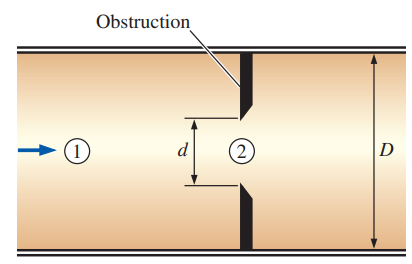
\includegraphics[width=0.2\textwidth]{Figures/Sec8 Obstruction Flowmeter.png}
    \caption{Obstruction flowmeter}
    \label{fig:obstruction_flowmeter}
\end{figure}
\begin{fleqn}
    \begin{align*}
        &\text{Obstruction flowmeter: } \dot{V} = A_0 C_d \sqrt{\frac{2(P_1 - P_2)}{\rho (1 - \beta^4)}} \\
        &\text{Mass Balance : } \implies \dot{x}_1 = (d/D)^2 \dot{x}_2 \\
        &\text{Head Loss: } h_L = \frac{P_1}{\rho g} + \frac{\dot{x}_1^2}{2g} + z_1 - \frac{P_2}{\rho g} - \frac{\dot{x}_2^2}{2g} - z_2 \\
    \end{align*}
\end{fleqn}
\section*{6. Momentum Analysis of Flow Systems}
\subsection*{6.1 General Procedure}
\begin{enumerate}
    \item Utilize the Bernoulli equation to obtain the $P_{1, \text{gage}}$
    \item $\sum \vec{F}$ represents external forces acting on the system. Some examples are:
    \begin{enumerate}[label=\roman*)]
        \item Pressure: $P_{1, \text{gage}} A_1$
        \item Reaction force: $F_{R}$
    \end{enumerate}
    \item Use momentum equation to obtain forces. For uniform flow, $\beta = 1$.  If not given, 
    it is expected to assume uniform flow.
\end{enumerate}

\subsection*{6.2 Variable Definitions}
\begin{itemize}
    \item $\beta$: Momentum-flux correction factor. It's a correction factor for the surface integral.
\end{itemize}

\subsection*{6.3 Formulas}
\begin{fleqn}
    \begin{align*}
        &\text{Momentum Equation: } \sum \vec{F} = \sum_{\text{out}} \beta \dot{m} \vec{V} - \sum_{\text{in}} \beta \dot{m} \vec{V} \\
        &\text{Momentum Correction Factor: } \beta = \begin{cases}
            4/3 & \text{laminar} \\
            1 & \text{turbulent}
        \end{cases} \\ 
    \end{align*}
\end{fleqn}
\section*{8. Internal Flow: Pipes and Ducts}
\subsection*{8.2 Variable Definitions}
\begin{itemize}
    \item Pressure drop: A pressure drop due to viscous effects represents an irreversible pressure loss
    \item Head loss: Additional height that the fluid needs to be raised by a pump in order to overcome the frictional losses in the pipe
    \item Major loss: The viscous (frictional) losses for fully-developed flow through straight pipe section
    \item Minor loss: Additional losses at the pipe. 
    \item $K_L$ = Loss coefficient
    \item $\alpha$ = Kinetic energy correction factor
\end{itemize}

\subsection*{8.3 Formulas}
\begin{align*}
    D_h &= \frac{4A_c}{\text{wetted perimeter}} \\
    \text{Re} &= \frac{\rho V D_h}{\mu} \\
    L_{h, \text{laminar}} &= 0.05 \text{Re} D \\
    L_{h, \text{turbulent}} &= 10D
\end{align*}
Pressure stuff
\begin{align*}
    \Delta P &= \frac{32 \mu L \dot{x}_{\text{avg}}}{D^2}, \; \text{Laminar} \\
    \Delta P_L &= f \frac{L}{D} \frac{\rho \dot{x}_{\text{avg}}^2}{2}, \; \text{Either} \\
    h_L &= f \frac{L}{D} \frac{\dot{x}_{\text{avg}}^2}{2g}, \; \text{Either} \\
    f &= \frac{8\tau_w}{\rho \dot{x}_{\text{avg}}^2} \overset{\text{laminar}}{=} \frac{64}{\text{Re}}
\end{align*}
Horizontal pipe, laminar (Re$<2300$):
\begin{align*}
    \dot{x}_{\text{avg}} &= \frac{\Delta P D^2}{32 \mu L} \\
    \dot{V}_{\text{avg}} &= \frac{\Delta P \pi D^4}{128 \mu L} 
\end{align*}
Turbulent flow through pipe:
\begin{align*}
    \frac{1}{\sqrt{f}} &= -2 \log_{10} \left(\frac{\epsilon}{3.7D} + \frac{2.51}{\text{Re} \sqrt{f}}\right) \\
\end{align*}    
Energy equation \textbf{($\alpha = 2$ for laminar, $\alpha = 1.05$ for turbulent)}
\begin{align*}
    \frac{P_1}{\rho g} + \alpha_1 \frac{\dot{x}_1^2}{2g} + z_1 + h_{\text{pump}, u} &= \frac{P_2}{\rho g} + \alpha_2 \frac{\dot{x}_2^2}{2g} + z_2 + h_{\text{turbine}, e} + h_L
\end{align*}
Loss coefficient
\begin{align*}
    h_{L, \text{minor}} = K_L \frac{\dot{x}^2}{2g}
\end{align*}
for sudden expansion,
\begin{align*}
    K_L = \alpha \left(1 - \frac{d_{\text{small}}}{d_{\text{large}}}\right)^2
\end{align*}
pump work,
\begin{align*}
    \dot{W}_{\text{pump}} = \dot{V} \Delta P
\end{align*}

\section*{9. Differential Analysis of Fluid Flow}
\subsection*{9.1 General Procedure}
\begin{enumerate}
    \item Most problems will be simplifiable to 2D or 1D because full form Navier-Stokes equations are too difficult to solve. The art of these 
    problems is to simplify the equations to a form that can be solved.
    \item Common assumptions are: steady, laminar, incompressible, constant viscosity, constant pressure, constant temperature, and
    parallel flow (velocity only in one direction). Gravity typically acts in the negative z-direction (unless it's like an inclined 
    plane where you'd set your coordinates to be tangential and normal to the plane).
    \item Check the problem statement for these key words: %steady, laminar, incompressible, constant density, constant viscosity, constant pressure,\
    \begin{enumerate}[label=\roman*)]
        \item Steady: All $\frac{\partial}{\partial t} = 0$
        \item Laminar: Generally implies parallel flow, flow in one direction only.
        \item Incompressible: $\text{div}(\vec{V}) = \nabla \cdot \vec{V} = 0$, $\frac{\partial \rho}{\partial t} = 0$
        \item Pressure acts in only one-direction: $\frac{\partial P}{\partial x} = 0$, $\frac{\partial P}{\partial y} = 0$, or $\frac{\partial P}{\partial z} = 0$ 
        \item Parallel flow: Velocity in the direction of motion is non-zero, velocity in the other directions is zero.
        \item Gravity only in z-direction: $\vec{g} = -g \hat{k}$
    \end{enumerate}
    \item Boundary conditions:
    \begin{enumerate}[label=\roman*)]
        \item No-slip: $\vec{V}_{\text{fluid}} = \vec{V}_{\text{boundary}}$ at an interface boundary.
        \item No-shear at a : $\tau_{\text{fluid}} = \tau_{\text{boundary}} \approx 0$ at a free surface boundary with small surface tension like air.
    \end{enumerate}
    \item Try to simplify the continuity equation first. Use the results in simplifying the Navier-Stokes equation.
    \item Solve for whatever is asked for in the problem statement.
\end{enumerate}

\subsection*{9.2. Operator Definitions}
\begin{itemize}
    \item $\nabla$: The gradient operator, $\nabla = \frac{\partial}{\partial x} \hat{i} + \frac{\partial}{\partial y} \hat{j} + \frac{\partial}{\partial z} \hat{k}$
    \item $\frac{\partial \vec{V}}{\partial x}$: The vector partial derivative, 
    $\frac{\partial \vec{V}}{\partial x} = \frac{\partial u}{\partial x} \hat{i} + \frac{\partial v}{\partial x} \hat{j} + \frac{\partial w}{\partial x} \hat{k}$
    \item $\frac{D}{Dt}$: The material derivative, $\frac{D \vec{T}}{Dt} = \frac{\partial \vec{T}}{\partial t} + (\vec{V} \cdot \nabla) \vec{T}$
    \footnote[1]{$(\vec{V} \cdot \nabla)$ is the convective derivative operator, not div($\vec{V}$)}
    \item $(\vec{V} \cdot \nabla)$: The convective derivative, $(\vec{V} \cdot \nabla) \vec{T} = u \frac{\partial \vec{T}}{\partial x} + v \frac{\partial \vec{T}}{\partial y} + w \frac{\partial \vec{T}}{\partial z}$
    \item $\nabla^2$: The Laplacian operator, $\nabla^2 = \frac{\partial^2}{\partial x^2} + \frac{\partial^2}{\partial y^2} + \frac{\partial^2}{\partial z^2}$
\end{itemize}

\subsection*{9.3 Variable Definitions}
\begin{itemize}
    \item $\vec{V}$: Velocity vector, $\vec{V} = u \hat{i} + v \hat{j} + w \hat{k}$
    \item $\rho$: Density
    \item $\mu$: Viscosity
    \item $P$: Pressure
\end{itemize}

\subsection*{9.4 Formulas}
\begin{fleqn}
\begin{align*}
    &\text{Continuity Equation: } \frac{\partial \rho}{\partial t} + \nabla \cdot (\rho \vec{V}) = 0 \\
    % &\text{Cartesian: } \frac{\partial \rho}{\partial t} + \frac{\partial}{\partial x}(\rho u) + \frac{\partial}{\partial y}(\rho v) 
    % + \frac{\partial}{\partial z}(\rho w) = 0 \\
    % &\text{Cylindrical: } \frac{\partial \rho}{\partial t} + \frac{1}{r} \frac{\partial(r \rho u)}{\partial r} + \frac{\partial(\rho v)}{\partial \theta} 
    % + \frac{\partial(\rho w)}{\partial z} = 0 \\
    &\text{Special Case 1: Steady Compressible Flow: } \nabla \cdot (\rho \vec{V}) = 0 \\
    &\text{Special Case 2: Incompressible Flow: } \nabla \cdot \vec{V} = 0 \\
    &\text{Incompressible flow, Newtonian, Navier-Stokes Equation:}
\end{align*}
\end{fleqn}
\begin{align*}
    \rho \frac{ D \vec{V}}{D t}  &= -\nabla P + \rho \vec{g} + \mu \nabla^2 \vec{V} 
\end{align*}
For example in x-direction:
\begin{align*}
    \rho \left(\frac{\partial u}{\partial t} + u \frac{\partial u}{\partial x} + v \frac{\partial u}{\partial y} + w \frac{\partial u}{\partial z}\right) 
    = &-\frac{\partial P}{\partial x} + \rho g_x \\
    &+ \mu \left(\frac{\partial^2 u}{\partial x^2} + \frac{\partial^2 u}{\partial y^2} + \frac{\partial^2 u}{\partial z^2}\right)
\end{align*}
\subsection*{9.5 General Terms}
\begin{itemize}
    \item Control volume analysis: very useful tool to engineering for flow analysis. Gives 'engineering analysis' answer, sometimes crude approximation, but always useful.
    A method of analysis in which a volume in space is selected and the conservation of mass, momentum, and energy are applied to the volume
    \item Differential analysis:  in principle can be used for any problems. In practice, limited cases where exact analytical solutions exist. 
    Nowadays, CFD (computational fluid dynamics) simulations are widely performed based on differential analysis. Involves application of differential 
    equations of fluid motion to any and every point in the flow field over a region called the flow domain.
    Experimental (dimensional) analysis: based on the results of experiments. Technique to derive the most use out of the fewest number of experiments 
    (which cost time and money)
\end{itemize}
\section*{10. Boundary Layer Approximation}
\subsection*{10.1 General Procedure}
\begin{enumerate}
    \item Identify the type of flow using the Reynolds number. If the Re $> 5 \times 10^5$, the flow is turbulent. If the Re $< 5 \times 10^5$, the flow is laminar.
    \item Use Table \ref{tab:boundary_layer_approximation} to determine whatever you need.
\end{enumerate}

\subsection*{10.2 Variable Definitions}

\subsection*{10.3 Formulas}
\begin{fleqn}
    \begin{align*}
        &\text{Reynolds Number: } \text{Re}_x = \frac{\rho V x}{\mu}  = \frac{V x}{\nu} \\
        &\text{Boundary Layer Thickness: } \frac{\delta}{x} = 4.91 \sqrt{\text{Re}_x} \\
        &\text{Wall Shear Stress: } \tau_w = \frac{0.332 \rho U^2}{\sqrt{\text{Re}_x}} \\
        &\text{Local Friction Coefficient: } C_f = \frac{\tau_w}{\frac{1}{2} \rho U^2} = \frac{0.664}{\sqrt{\text{Re}_x}} \\
        &\text{Displacement Thickness: } \delta^* = \int_0^\infty \left(1 - \frac{u}{U}\right) dy = \frac{1.72 x}{\sqrt{\text{Re}_x}} \\
        &\text{Momentum Thickness: } \theta = \int_0^\infty \frac{u}{U} \left(1 - \frac{u}{U}\right) dy = \frac{0.664 x}{\sqrt{\text{Re}_x}} \\   
        &\text{Drag Force: } F_D = \int_A \tau_w dA = \int_0^L \tau_w w dx \\
        &\text{Continuity Equation: } \frac{\partial u}{\partial x} + \frac{\partial v}{\partial y} = 0 \\
        &\text{Momentum Equation: } u \frac{\partial u}{\partial x} + v \frac{\partial u}{\partial y} = U \frac{dU}{dx} + \nu \frac{\partial^2 u}{\partial y^2} \\
    \end{align*}
\end{fleqn}

\begin{table}[H]
    \caption{Boundary Layer Approximation}
    \label{tab:boundary_layer_approximation}
    \centering
    \begin{tabular}{ccc}
        \hline
        Property & Laminar & Turbulent \\
        \hline
        Boundary Layer Thickness & $\frac{\delta}{x} = 4.91 \sqrt{\text{Re}_x}$ & $\frac{\delta}{x} = \frac{0.16}{(\text{Re}_x)^{1/7}}$ \\
        Displacement Thickness & $\frac{\delta^*}{x} = \frac{1.72}{\sqrt{\text{Re}_x}}$ & $\frac{\delta^*}{x} = \frac{0.020}{(\text{Re}_x)^{1/7}}$ \\
        Momentum Thickness & $\frac{\theta}{x} = \frac{0.664}{\sqrt{\text{Re}_x}}$ & $\frac{\theta}{x} = \frac{0.016}{(\text{Re}_x)^{1/7}}$ \\   
        Local Friction Coefficient & $C_f = \frac{0.664}{\sqrt{\text{Re}_x}}$ & $C_f = \frac{0.027}{(\text{Re}_x)^{1/7}}$ \\
        Wall Shear Stress & $\tau_w = \frac{0.332 \rho U^2}{\sqrt{\text{Re}_x}}$ & $\tau_w = \frac{0.013 \rho U^2}{(\text{Re}_x)^{1/7}}$ \\
        \hline
    \end{tabular}
\end{table}
\section*{Terms}
% Static Pressure: the actual thermodynamic pressure dynamic Pressure: represents the pressure rise when fluid motion is brought to a stop isentropically Hydrostatic pressure: value depends on the reference level selected where z=0. A ‘potential’ pressure. Total Pressure = static pressure + dynamic pressure hydrostatic pressure. Stagnation pressure= static pressure+dynamic pressure. Pressure head: height of fluid needed to produce a static pressure P velocity head: height of fluid needed to produce velocity V during a free, frictionless vertical fall. Elevation head: height relative to some reference plate z=0. Hydraulic Grade Line(HGL): the line that represents pressure and elevation heads.Energy Grade Line (EGL): the line that represents the total head. Obstruction flow meters: obstruction flow meters intentionally constrict the flow, and measure the drop in static pressure at the constriction. This pressure drop is proportional to the flow velocity through the constriction. Control volume analysis: very useful tool to engineering for flow analysis. Gives ‘engineering analysis’ answer, sometimes crude approximation, but always useful. Differential (small-scale) analysis: in principle can be used for any problems. In practice, limited cases where exact analytical solutions exist. Nowadays, CFD (computational fluid dynamics) simulations are widely performed based on differential analysis. Experimental (dimensional) analysis: based on the results of experiments. Technique to derive the most use out of the fewest number of experiments (which cost time and money). Displacement thickness: the distance that a streamline just outside the boundary layer is deflected away from the wall due to the effect of the boundary layer. The imaginary increase in the thickness of the wall, as seen by the outer flow due to the effect of the growing boundary layer. Momentum thickness: a measure of the loss of momentum flux per unit width. Thickness of a 
% layer of fluid velocity U for which the momentum flux is equal to the deficit of momentum flux through the boundary layer. 


%Momentum thickness is defined as the loss of momentum flux per unit width divided by 𝝆U^2 due to the presence of the growing boundary layer. 𝝆U^2𝜃 the loss of momentum flux per unit width due to the growing boundary layer.
\begin{itemize}
    \item Static Pressure: the actual thermodynamic pressure
    \item Dynamic Pressure: represents the pressure rise when fluid motion is brought to a stop isentropically
    \item Hydrostatic pressure: value depends on the reference level selected where z=0. A 'potential' pressure.
    \item Total Pressure = static pressure + dynamic pressure hydrostatic pressure.
    \item Stagnation pressure= static pressure+dynamic pressure.
    \item Pressure head: height of fluid needed to produce a static pressure P
    \item Velocity head: height of fluid needed to produce velocity V during a free, frictionless vertical fall.
    \item Elevation head: height relative to some reference plate z=0.
    \item Hydraulic Grade Line(HGL): the line that represents pressure and elevation heads.
    \item Energy Grade Line (EGL): the line that represents the total head.
    \item Obstruction flow meters: obstruction flow meters intentionally constrict the flow, and measure the drop in static pressure at the constriction. This pressure drop is proportional to the flow velocity through the constriction.
    \item Control volume analysis: very useful tool to engineering for flow analysis. Gives 'engineering analysis' answer, sometimes crude approximation, but always useful.
    \item Differential (small-scale) analysis: in principle can be used for any problems. In practice, limited cases where exact analytical solutions exist. Nowadays, CFD (computational fluid dynamics) simulations are widely performed based on differential analysis.
    \item Experimental (dimensional) analysis: based on the results of experiments. Technique to derive the most use out of the fewest number of experiments (which cost time and money).
    \item Displacement thickness: the distance that a streamline just outside the boundary layer is deflected away from the wall due to the effect of the boundary layer. The imaginary increase in the thickness of the wall, as seen by the outer flow due to the effect of the growing boundary layer
    \item Momentum thickness: defined as the loss of momentum flux per unit width divided by $\rho U^2$ due to the presence of the growing boundary layer. $\rho U^2 \theta$ the loss of momentum flux per unit width due to the growing boundary layer.
\end{itemize}


\end{multicols}

\end{document}
